\subsection{\href{https://www.disenioconingenio.com.ar}{disenioconingenio}}
   \hypertarget{subsec:dci}
   Durante la dirección de la empresa disenioconingenio, se desarrollaron varios productos para la venta en mercado y customizados de acuerdo a características requeridas por los clientes, se destacan los siguientes:

   \cvlistitem{RFID 125Khz Multiprotocolo}
   Se diseño un novedoso lector de tarjetas RFID en la frecuencia de 125Khz totalmente con un frontend discreto y totalmente decodificado por el microcontrolador. Esto permite leer tarjetas de diferentes fabricantes y diferentes protocolos, y combinarlo con salidas de datos multiples, como RS232, RS485, Wiegand, ABA, etc. 
   Se muestran algunas fotos del producto en la figura \ref{fig:rfid}.
   \begin{figure}
      \begin{center}
         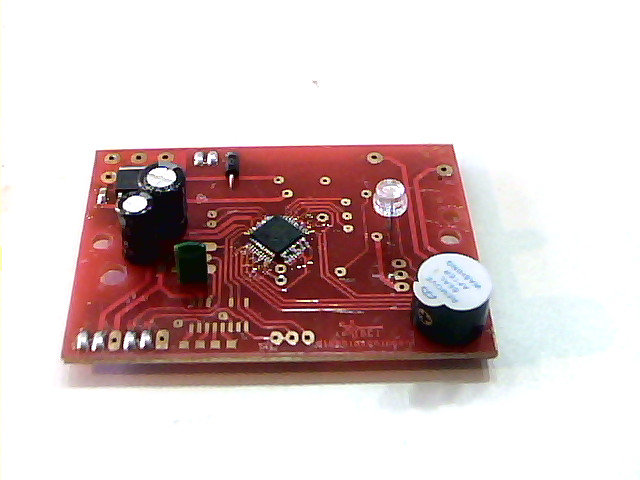
\includegraphics[width=0.24\textwidth]{portfolio/rfid5.jpg}
         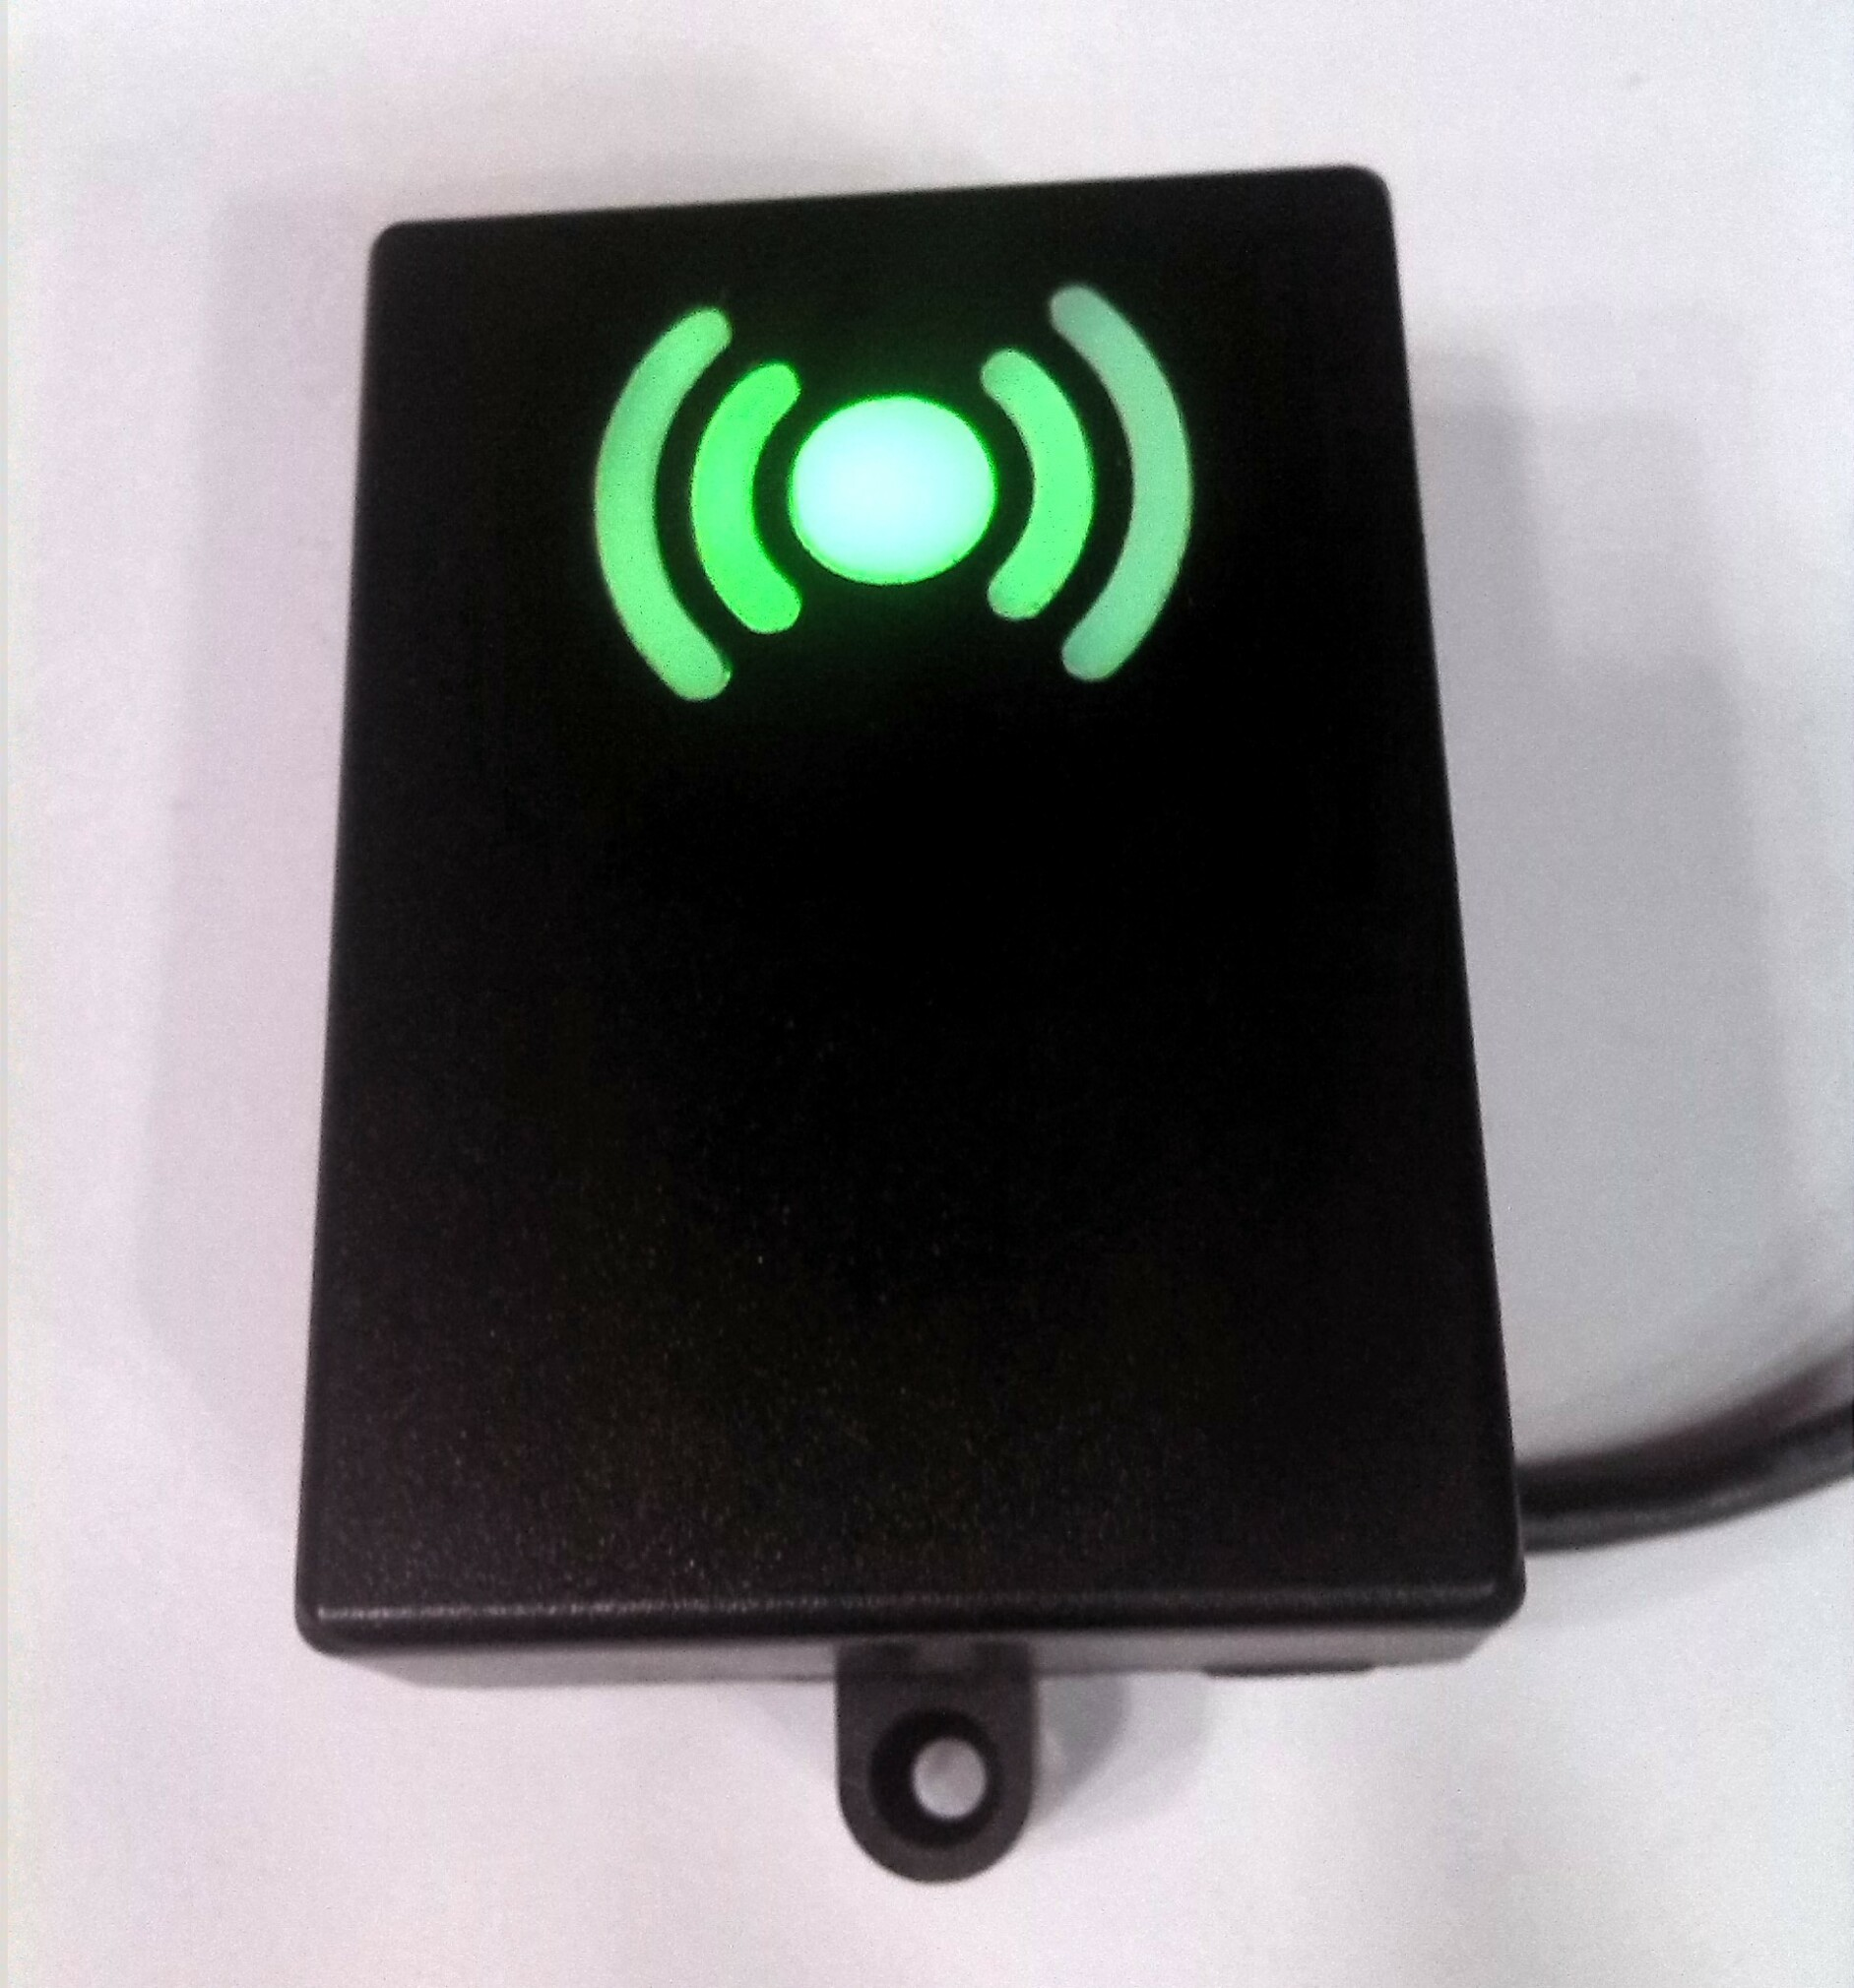
\includegraphics[width=0.24\textwidth]{portfolio/rfid2.jpg}
         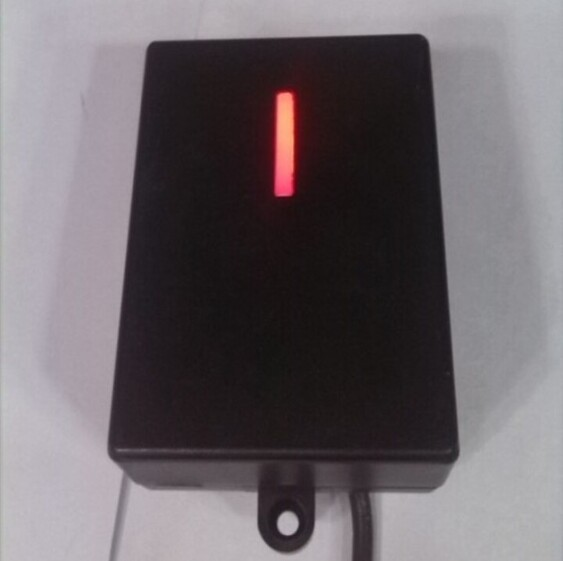
\includegraphics[width=0.24\textwidth]{portfolio/rfid3.jpg}
         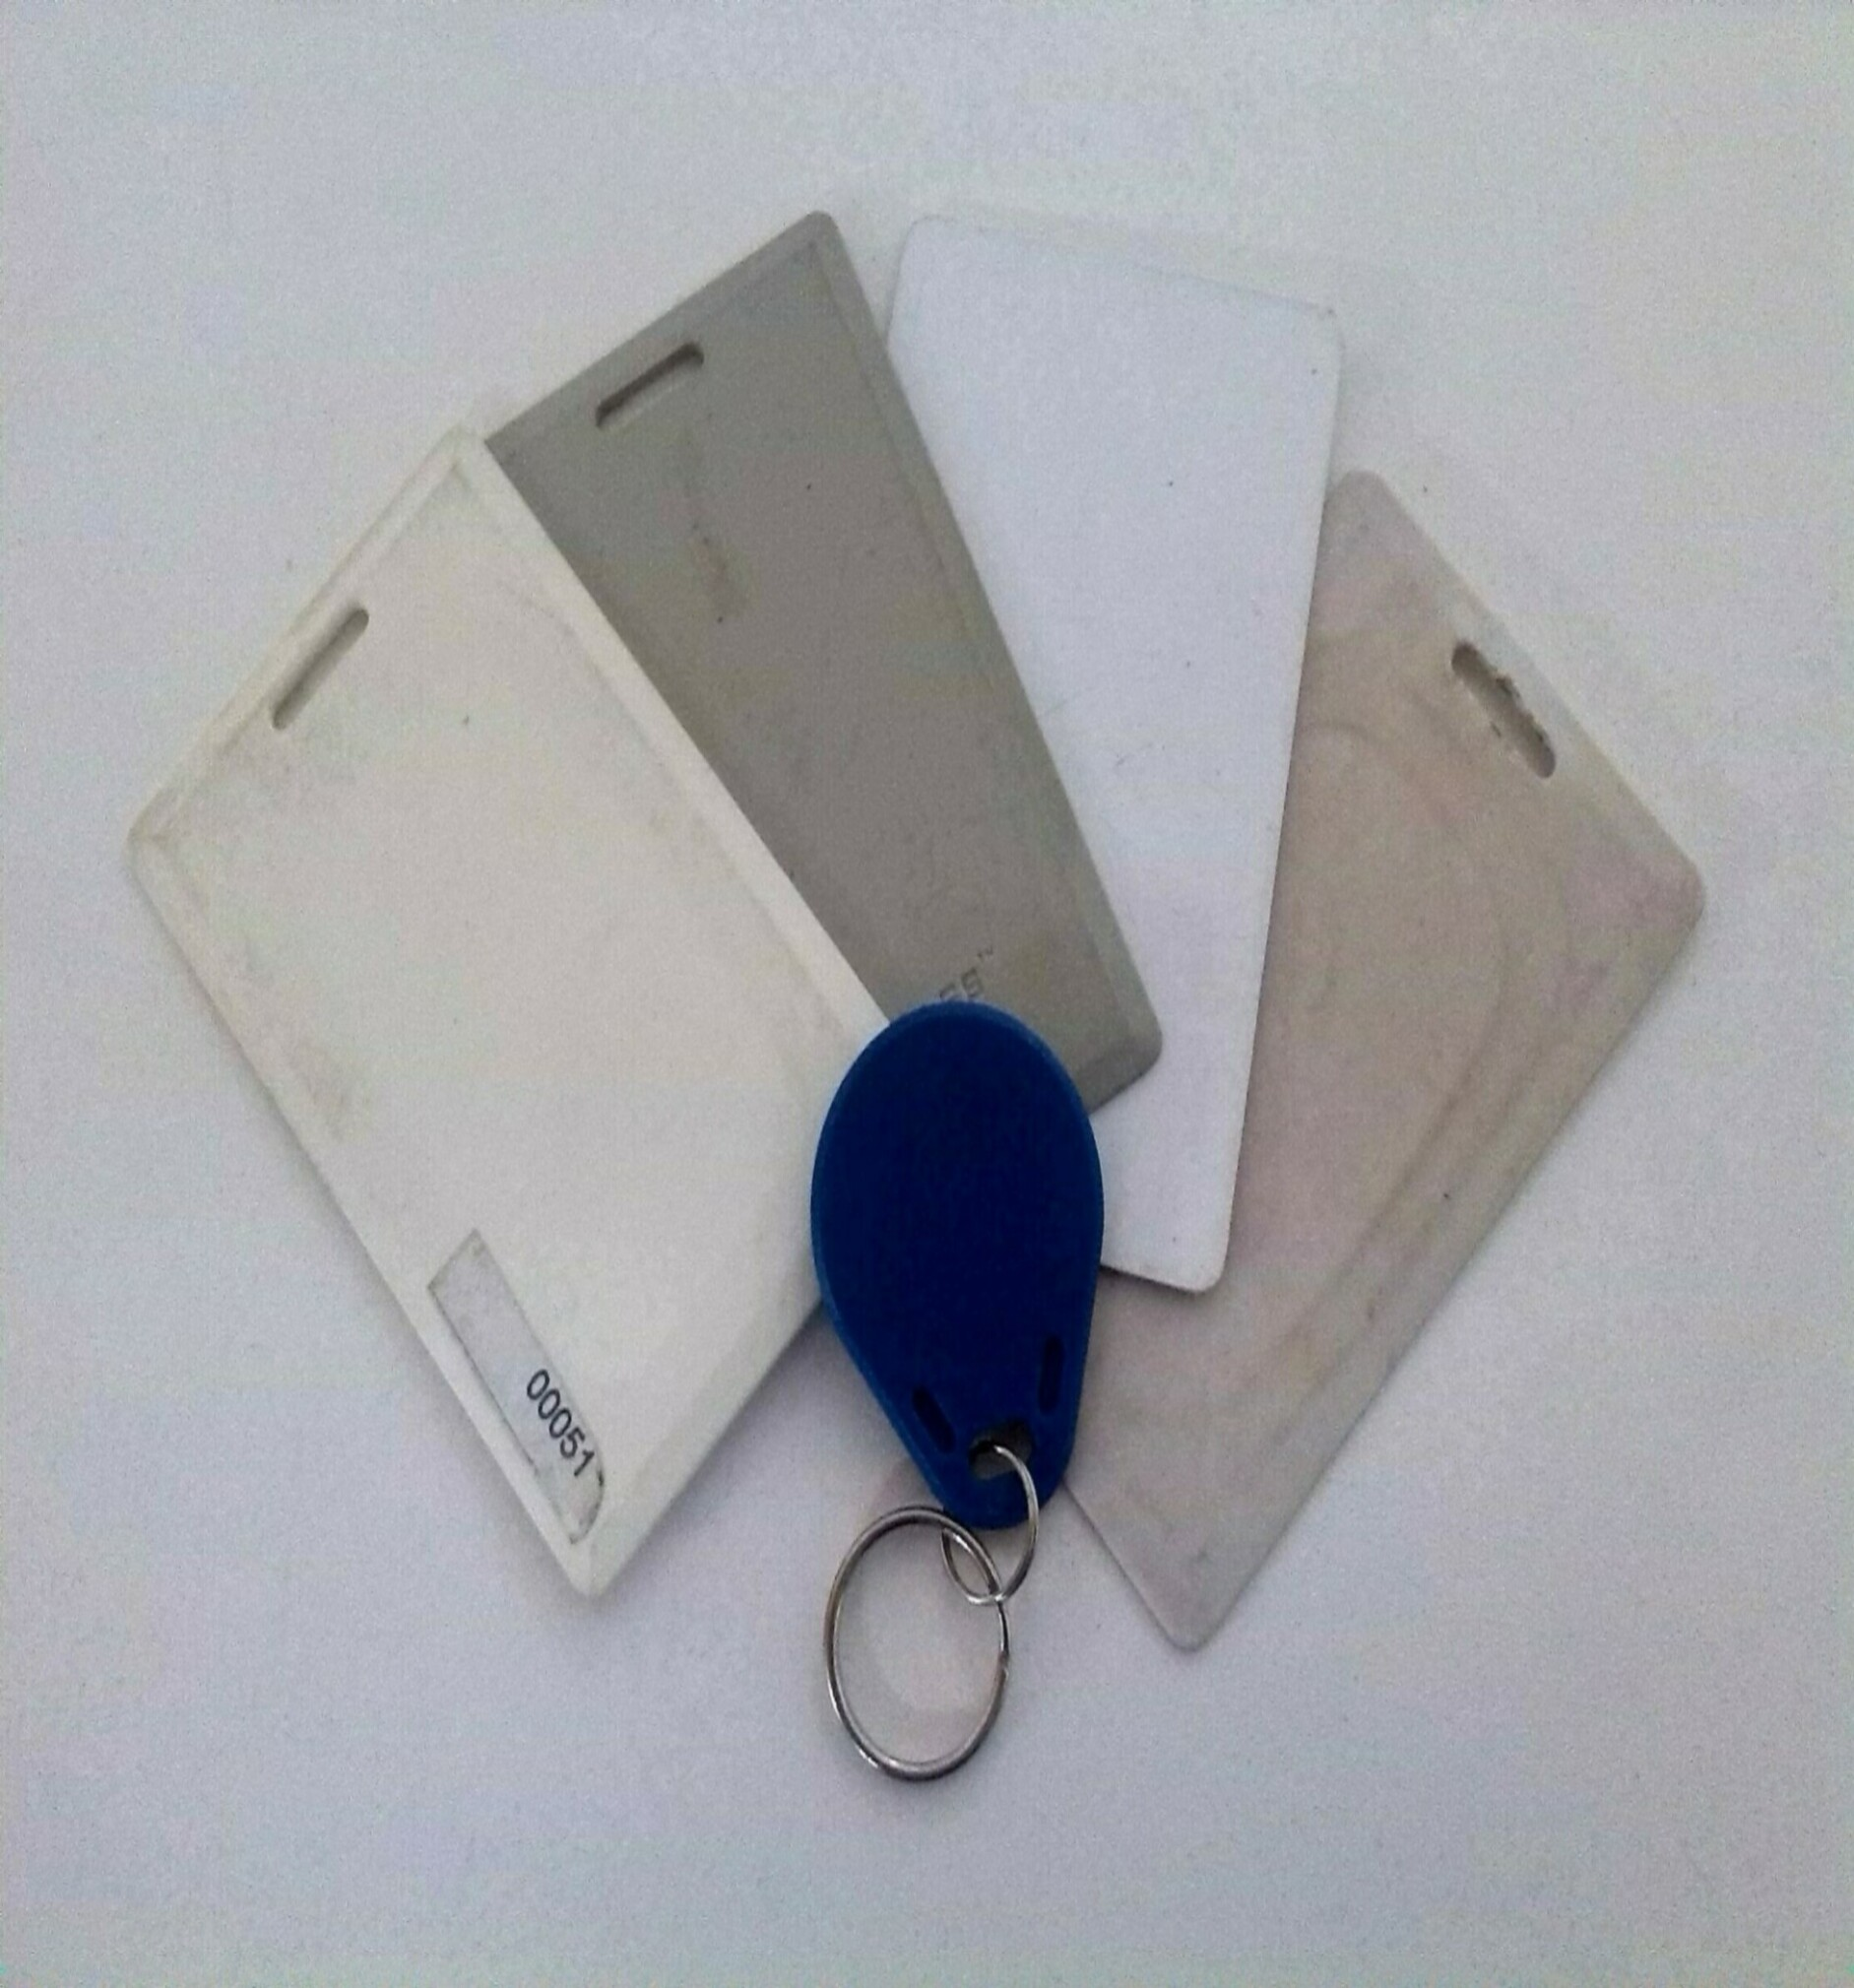
\includegraphics[width=0.24\textwidth]{portfolio/rfid4.jpg}
      \end{center}
      \caption{Lector RFID 125khz mutiprotocolo de tarjetas y de salida de datos, compatible con la mayoría de los fabricantes de tarjetas.}
      \label{fig:rfid}
   \end{figure}


   \cvlistitem{Hango - Motorizador para silla de ruedas}
   En conjunto con instituciones dedicadas a la asistencia a personas con dificultades motrices como CIAPAT, AEDIN y FAME, se obtuvo la experiencia y requerimientos para poder desarrollar Hango.\\
      Consiste en un motorizador que se acopla a las sillas de ruedas propulsadas manualmente otorgando comodidad e independencia.
Se desarrollaron modelos para niños y adultos hasta 100kg con diferentes estilos de comandos, algunos basados en el típico joystick, y otros mas novedosos usando la tecnología de pantalla táctil que no solo ofrece comodidad sino que permite mover la silla a pacientes con dificultades para mover un joystick convencional. \\
El equipo se adapta a la gran mayoría de las sillas de mercado con una mínima intervención mecánica y permite el acople y desacople sin herramientas, adecuado para traslados en coche, avión, etc.\\
Se pueden ver algunas fotos de la silla y sus partes en la figuras \ref{fig:hango1} y \ref{fig:hango2} y también videos del equipo en funcionamiento en el siguiente link \href{https://www.youtube.com/watch?v=6DcVH3cskDw&list=PLW6TA4Tyq4ZQ31ItL6zjCoVH7Mv3uosIi}{video Hango}

   \begin{figure}
      \begin{center}
         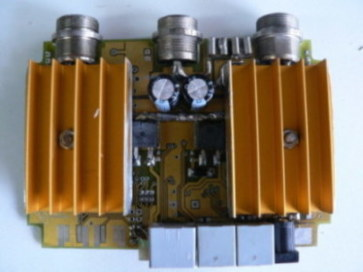
\includegraphics[width=0.24\textwidth]{portfolio/hango1.jpg}
         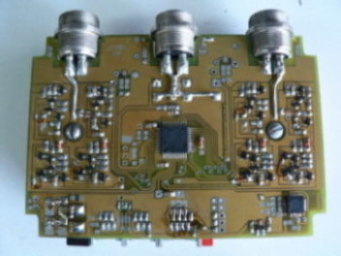
\includegraphics[width=0.24\textwidth]{portfolio/hango2.jpg}
         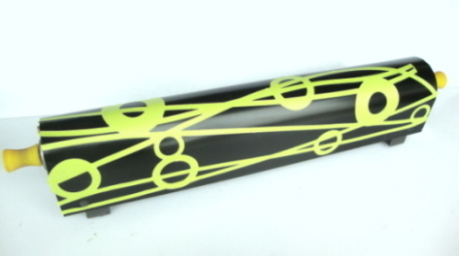
\includegraphics[width=0.24\textwidth]{portfolio/hango3.jpg}
         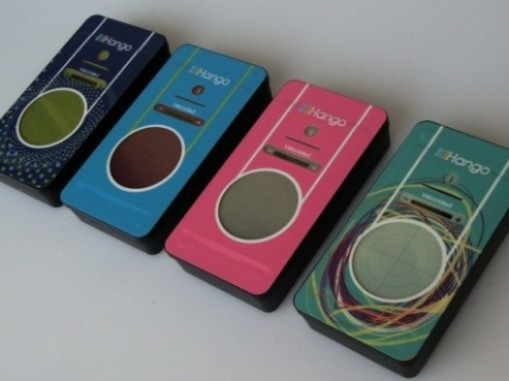
\includegraphics[width=0.24\textwidth]{portfolio/hango4.jpg}
      \end{center}
      \caption{Placas de potencia, modulo motorizador y comandos de Hango}
      \label{fig:hango1}
   \end{figure}
   \begin{figure}
      \begin{center}
         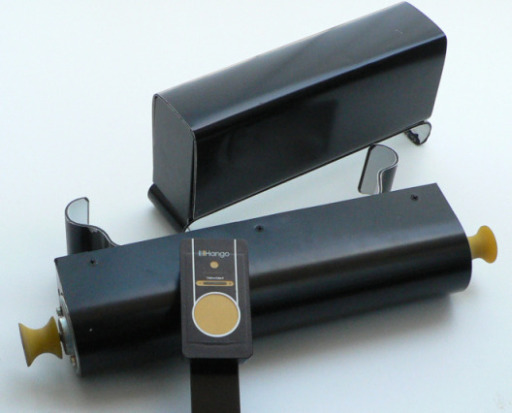
\includegraphics[width=0.24\textwidth]{portfolio/hango5.jpg}
         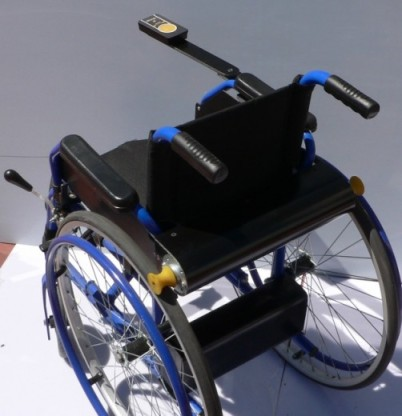
\includegraphics[width=0.24\textwidth]{portfolio/hango6.jpg}
         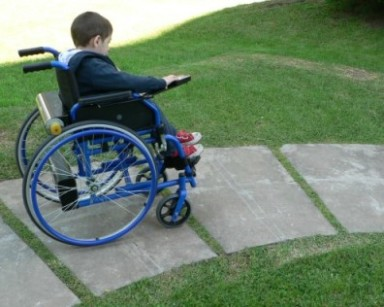
\includegraphics[width=0.24\textwidth]{portfolio/hango7.jpg}
         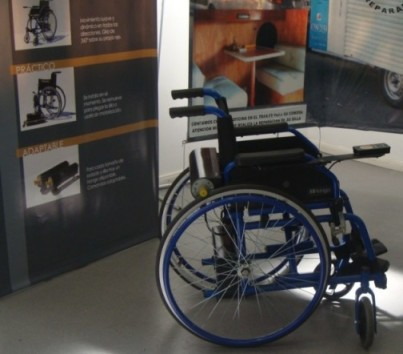
\includegraphics[width=0.24\textwidth]{portfolio/hango8.jpg}
      \end{center}
      \caption{Hango, despiece de partes, silla de niños con Hango y exposición en la que participo.}
      \label{fig:hango2}
   \end{figure}
